% Chapter 1

\chapter{Background} % Main chapter title

\label{back} % For referencing the chapter elsewhere, use \ref{Chapter1}

\lhead{Chapter 2. \emph{
Background}} % This is for the header on each page - perhaps a shortened title
The present work relied in two important concepts: gamification and spaced repetition. An overview of both concepts sets the scenario for the proposed solution. Gamification provides an alternative to improve user's experience, whereas spaced repetition offers a way to ease the retention of new knowledge. Among the several alternatives that implement spaced repetition, Anki and its mobile interface, AnkiDroid, provide a general approach with a large user base. In addition, casual games offer characteristics that make them adaptble to non leisure contexts including learning. Finally, the popularity of 2048 game has turned it into a subject of several studies.

%----------------------------------------------------------------------------------------
\section{Gamification}
Gamification can be defined as the process of adding game elements and mechanics in non-game contexts \citep{deterding2011game}. The main objective of Gamification is to improve the user's experience and increase the motivation to use a product or service. To accomplish such objective, Gamification takes advantage of the inherent nature of humans to play. Unlike mandatory activities such study and work, play is voluntary and free; its main outcome is a feeling of joy and excitement \citep{johan1950homo}. These conditions set the environment for the adoption of game concepts and techniques in broader contexts.

Over the past ten years, Gamification has attracted the attention of industry and academia. In the industry, companies have found a means to improve the performance and commitment of employees by avoiding traditional schemes of monetary rewards and punishments. Morevover, Gamification provides a set of tools to increase the loyalty and engagement of users and customers. For the academia, Gamification has expanded and merged various field of research given its interdisciplinary nature. It has attracted the attention of researchers in areas such as Human Computer Interaction, Software Development, Psychology, Pedagogy, Bussiness Management and others.

%----------------------------------------------------------------------------------------
\section{Spaced Repetition}
Spaced Repetition is a technique that facilitates the retention of new knowledge. It leverages the spacing effect phenomenon to help learners memorize specific contents \citep{hintzman1974theoretical}. This phenomenon allows learners to increase their capacity of retention by acquiring new knowledge in short recurrent sessions rather than in a single massive revision. In its basic form, Spaced Repetition sets increasing intervals of time between subsequent review sessioins of previously learned material. This means that the more challenging the content, the more frequently is reviewed by a learner. Then, the frequency of repetition is adjusted as the learner progresses.

Among the various existing techniques for memorization, Spaced Repetition stands out due to its simplicity and flexibility. The duration of each revision along with the inteval time between consecutive sessions is defined by the learner. In addition, the learner assesses the easiness of the content under revision to determine the frequency of repetition. Finally, Spaced Repetition is a technique that can be used to learn new content from any field, but it is specially useful when the number of items to memorize is large. Such characteristics allow the implementation of this technique as a piece of software, making it available to a wider audience.

%----------------------------------------------------------------------------------------
\section{AnkiDroid}
Anki is a platform that implements a general solution for spaced repetition. Thus, it can be used to learn and memorize content from any field. Its community has created an extense content base in a multitude of categories including languages, art, science and trivia. It provides several interfaces including a desktop applications for Linux, Mac and Windows. In mobile environments, it provides applications for iOS and Android devices. The version for Android devices is known as AnkiDroid which code is publicly available under the GNU general public license.

AnkiDroid has well defined logic and visual structures that implement most of the features presented in the desktop applications including creation and editing of flashcards, synchronization with the Anki system to save progress, and statistics of use. Moreover, it has been designed to be compatible with the majority of Android versions. Therefore, the application is available for a wide range of devices which have helped to increase its popularity as an educational tool as seen in Figure \ref{fig:anki-evolution}.

Moreover, AnkiDroid has a extense community of members that collaborate, support, and promote the use and development the application in web forums and groups. In regards to its development, the structure of its code allows modifications in the application that add or remove new features. The application can be modified to connect to external services, collect information of use, or include new elements. These characteristics have allowed to that an extense number of contributors (131) be part of its development.

\begin{figure}[htb]
    \vskip 5mm
        \begin{center}
            \includegraphics[scale=0.4]{./Figures/anki_progress.jpg}
            \caption{Evolution of the number of installations of AnkiDroid. Image taken from the twitter account of AnkiDroid (https://twitter.com/AnkiDroid)}
            \label{fig:anki-evolution}
        \end{center}
    \vskip -5mm
\end{figure}


%----------------------------------------------------------------------------------------
\section{Casual Video Games}
Casual video games, or casual games for short, are a category of digital games. The Casual Games Association (CGA) provides a definition based on the characteristics that a game needs to have to be considered casual. A casual game has to be fun, it needs to provide a quick way to access, and the gameplay must be easy to understand. These characteristics mean that users do not require any previous expertise or skills related to video games. For these reasons, casual games have a broad audience that includes people from all age groups.

The characteristics of this type of games have been leverage to adapt them to non leisure contexts including health and learning. In the health context, the use of casual games has been studied as an alternative element to improve mood and decrease stress \citep{russoniello2009effectiveness}. Additional studies have demonstrated the effectiveness of playing casual games as a recovery strategy after periods of high work strain \citep{reinecke2009games}. Finally, casual games have also been studied as educational tools \citep{peirce2010personalised}

%----------------------------------------------------------------------------------------
\section{2048 Game}
2048 game \citep{uberspot2017game} is a casual game with a 4x4 grid as seen in Figure \ref{fig:2048-grid}. The objective of the game is to merge numbered blocks until create one with the value 2048. The game starts with two blocks of value 2 which are randomly positioned in the grid. The player has to slide the blocks horizontally or vertically. The blocks move in the choosen direction; a block stops if it reaches an edge of the grid or collides with another block. If two colliding blocks have the same number, they are merged into a single block which value is the sum of the values of the forming blocks. In every turn, a new block of value 2 is randomly positioned in the grid.

\begin{figure}[htb]
    \vskip 5mm
        \begin{center}
            \includegraphics[scale=0.5]{./Figures/game_grid.png}
            \caption{Grid of the 2048 game.}
            \label{fig:2048-grid}
        \end{center}
    \vskip -5mm
\end{figure}

The poppularity of the game has turned it into a subject of different types of studies. The majority of these studies aim to analyse the game from the computational complexity perspective \citep{abdelkader20162048}, and propose several alternatives to win the game including neural networks \citep{boris2016evolving} and Monte-Carlo methods \citep{rodgers2014investigation}. However, the game has also been studied as an educational element to engage student interest \citep{neller2015pedagogical}

% % Add to description of game
%  the state of the grid is defined by the positions of the blocks and their values at a given turn
